\documentclass[10pt,a4paper]{article}
\usepackage[utf8]{inputenc}

% Define the page margin
\usepackage[margin=3cm]{geometry}

% Better typography (font rendering)
\usepackage{microtype}

% Math environments and macros
\usepackage{amsmath}
\usepackage{amsfonts}
\usepackage{amssymb}
\usepackage{amsthm}

% Define \includegraphics to include graphics
\usepackage{graphicx}

% Draw graphics from a text description
\usepackage{tikz}

% Syntax highlighting
\usepackage{minted}

% Set global minted options
\setminted{linenos, autogobble, frame=lines, framesep=2mm}

% Import the comment environment for orgtbl-mode
\usepackage{comment}

% Do not indent paragraphs
\usepackage{parskip}

\title{Virtual Physics, Sheet 5}
\author{Marten Lienen (03670270)}

\begin{document}

\maketitle

\section*{Exercise A}

We use the following variable assignments.

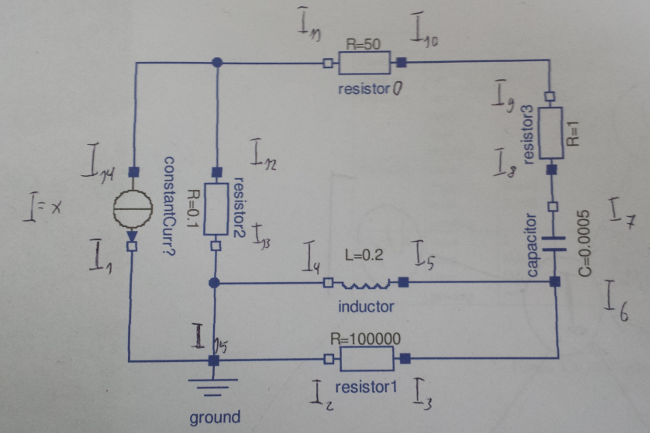
\includegraphics[width=\textwidth]{sheet-5/A}

\subsection*{Kirchhoff's First Law}

\begin{equation*}
  I_{1} + I_{2} + I_{4} + I_{13} + I_{15} = 0
\end{equation*}
\begin{equation*}
  I_{3} + I_{5} + I_{6} = 0
\end{equation*}
\begin{equation*}
  I_{7} + I_{8} = 0
\end{equation*}
\begin{equation*}
  I_{9} + I_{10} = 0
\end{equation*}
\begin{equation*}
  I_{11} + I_{12} + I_{14} = 0
\end{equation*}

\subsection*{Kirchhoff's Second Law}

\begin{equation*}
  U_{1} = U_{2} = U_{4} = U_{13} = U_{15}
\end{equation*}
\begin{equation*}
  U_{3} = U_{5} = U_{6}
\end{equation*}
\begin{equation*}
  U_{7} = U_{8}
\end{equation*}
\begin{equation*}
  U_{9} = U_{10}
\end{equation*}
\begin{equation*}
  U_{11} = U_{12} = U_{14}
\end{equation*}

\subsection*{Component Equations}

\subsubsection*{Current Source}

\begin{equation*}
  U_{1} - U_{14} = I \cdot (R_{0} + R_{1} + R_{3})
\end{equation*}
\begin{equation*}
  I_{1} = -I_{14} + I
\end{equation*}

\subsubsection*{Resistor 0}

\begin{equation*}
  U_{11} - U_{10} = R_{0} \cdot I_{10}
\end{equation*}
\begin{equation*}
  I_{11} = -I_{10}
\end{equation*}

\subsubsection*{Resistor 1}

\begin{equation*}
  U_{3} - U_{2} = R_{1} \cdot I_{2}
\end{equation*}
\begin{equation*}
  I_{3} = -I_{2}
\end{equation*}

\subsubsection*{Resistor 2}

\begin{equation*}
  U_{13} - U_{12} = R_{2} \cdot I_{13}
\end{equation*}
\begin{equation*}
  I_{13} = -I_{12}
\end{equation*}

\subsubsection*{Resistor 3}

\begin{equation*}
  U_{9} - U_{8} = R_{3} \cdot I_{8}
\end{equation*}
\begin{equation*}
  I_{9} = -I_{8}
\end{equation*}

\subsubsection*{Capacitor}

\begin{equation*}
  C \cdot \frac{\text{d}U_{C}}{\text{d}t} = I_{6}
\end{equation*}
\begin{equation*}
  U_{7} = U_{6} + U_{c}
\end{equation*}
\begin{equation*}
  I_{7} = -I_{6}
\end{equation*}

\subsubsection*{Inductor}

\begin{equation*}
  \frac{\text{d}I_{4}}{\text{d}t} \cdot L = U_{5} - U_{4}
\end{equation*}
\begin{equation*}
  I_{5} = -I_{4}
\end{equation*}

\subsubsection*{Ground}

\begin{equation*}
  U_{15} = 0
\end{equation*}

\section*{Exercise B}

We start with forward causalization to reduce the number of variables.
Replacing all voltages with the variable of lowest index results in
\begin{equation*}
  I_{1} + I_{2} + I_{4} + I_{13} + I_{15} = 0
\end{equation*}
\begin{equation*}
  I_{3} + I_{5} + I_{6} = 0
\end{equation*}
\begin{equation*}
  I_{7} = -I_{8}
\end{equation*}
\begin{equation*}
  I_{9} = -I_{10}
\end{equation*}
\begin{equation*}
  I_{11} + I_{12} + I_{14} = 0
\end{equation*}
\begin{equation*}
  I_{1} = -I_{14} + I
\end{equation*}
\begin{equation*}
  I_{11} = -I_{10}
\end{equation*}
\begin{equation*}
  I_{3} = -I_{2}
\end{equation*}
\begin{equation*}
  I_{13} = -I_{12}
\end{equation*}
\begin{equation*}
  I_{9} = -I_{8}
\end{equation*}
\begin{equation*}
  I_{7} = -I_{6}
\end{equation*}
\begin{equation*}
  I_{5} = -I_{4}
\end{equation*}
\begin{equation*}
  U_{1} - U_{11} = I \cdot (R_{0} + R_{1} + R_{3})
\end{equation*}
\begin{equation*}
  U_{11} - U_{9} = R_{0} \cdot I_{10}
\end{equation*}
\begin{equation*}
  U_{3} - U_{1} = R_{1} \cdot I_{2}
\end{equation*}
\begin{equation*}
  U_{1} - U_{11} = R_{2} \cdot I_{13}
\end{equation*}
\begin{equation*}
  U_{9} - U_{7} = R_{3} \cdot I_{8}
\end{equation*}
\begin{equation*}
  U_{7} = U_{3} + U_{c}
\end{equation*}
\begin{equation*}
  U_{1} = 0
\end{equation*}
\begin{equation*}
  C \cdot \frac{\text{d}U_{C}}{\text{d}t} = I_{6}
\end{equation*}
\begin{equation*}
  \frac{\text{d}I_{4}}{\text{d}t} \cdot L = U_{3} - U_{1}
\end{equation*}

Some simple eliminations yield

\begin{equation*}
  I_{13} = \frac{I \cdot (R_{0} + R_{1} + R_{3})}{R_{2}}
\end{equation*}
\begin{equation*}
  I_{6} = I_{14} - \frac{I \cdot (R_{0} + R_{1} + R_{3})}{R_{2}}
\end{equation*}
\begin{equation*}
  I_{1} = -I_{14} + I
\end{equation*}
\vspace{2em}
\begin{equation*}
  I_{14} = I_{2} + I_{4} + \frac{I \cdot (R_{0} + R_{1} + R_{3})}{R_{2}}
\end{equation*}
\begin{equation*}
  I_{15} = -I
\end{equation*}
\begin{equation*}
  U_{3} = R_{1} \cdot I_{2}
\end{equation*}
\begin{equation*}
  U_{7} = R_{1} \cdot I_{2} + U_{c}
\end{equation*}
\begin{equation*}
  U_{9} = -R_{0} \cdot \left( I_{2} + I_{4} \right) - I \cdot (R_{0} + R_{1} + R_{3})
\end{equation*}
\begin{equation*}
  I_{2} = \frac{\text{d}I_{4}}{\text{d}t} \cdot \frac{L}{R_{1}}
\end{equation*}
\begin{equation*}
  U_{c} = -\left( R_{0} + R_{1} + R_{3} \right)\frac{\text{d}I_{4}}{\text{d}t} \cdot \frac{L}{R_{1}} - \left( R_{3} + R_{0} \right)I_{4} - I \cdot (R_{0} + R_{1} + R_{3})
\end{equation*}
\begin{equation*}
  I_{4} = C \cdot \frac{\text{d}U_{C}}{\text{d}t} - \frac{\text{d}I_{4}}{\text{d}t} \cdot \frac{L}{R_{1}}
\end{equation*}

\end{document}
